\documentclass{article}

\usepackage{graphicx} % Required for inserting images
\usepackage{verbatim}
\usepackage[utf8]{inputenc}
\usepackage{graphicx}
\usepackage{float}
\usepackage{fancyvrb}
\usepackage{varwidth}
\usepackage{amsmath}
\usepackage{siunitx}



\title{Speech Processing\\EE679}
\author{Mohit\\20D070052 }
\date{October 2023}

\begin{document}

\maketitle
\begin{figure}[H]
\begin{center}

\includegraphics[scale = 0.2]{LOGO.jpeg}
\end{center}
\end{figure}
\section{Student Details}
\begin{tabular}{ l l  }
 Name: & Mohit \\ 
 Roll No: & 20D070052  \\  
\end{tabular}

\newpage

\section{Question 1}

Apply pre-emphasis to the signal.

\subsection{Solution 1}
Pre-emphasis is used as a high-pass filter with the formula P(z) = 1- az-1, where 'a' is a parameter, to slightly uniformalize the spectrum of the voice input, here I have used 0.97 as default value


\subsection{Code}
The code files are included in the .ipynb file included in the submission.

\subsection{Plots}

\begin{figure}[H]
\begin{center}
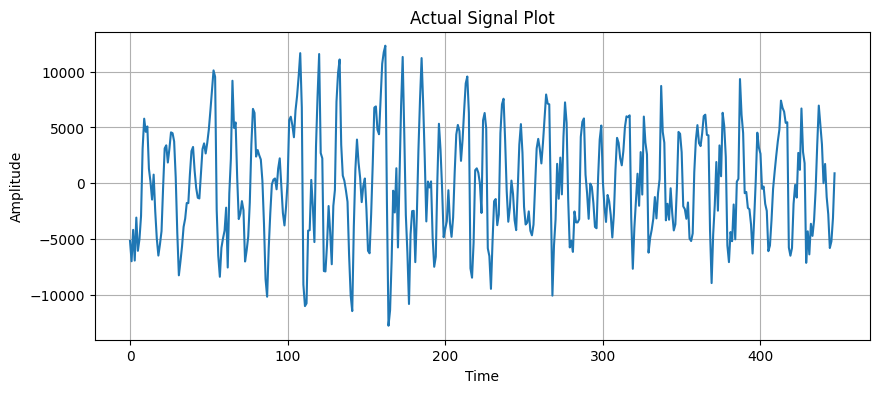
\includegraphics[scale = 0.5]{actual.png}
\end{center}
\end{figure}

\begin{figure}[H]
\begin{center}
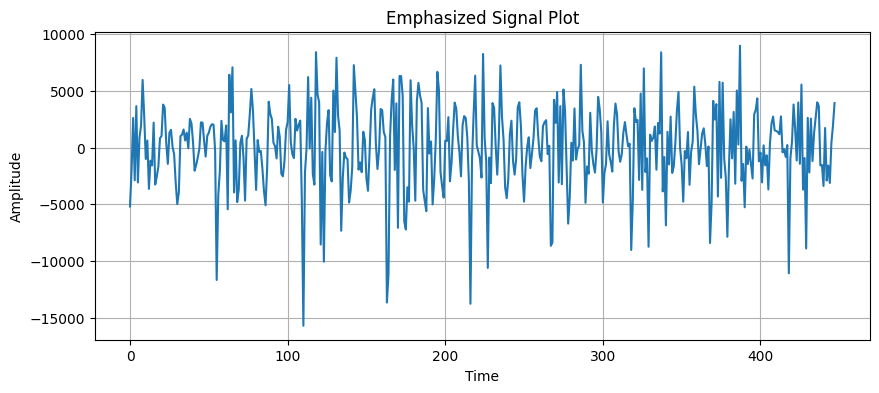
\includegraphics[scale = 0.5]{emph.png}
\end{center}
\end{figure}


\section{Question 2}

Next, compute and plot a single narrowband magnitude spectrum slice using a Hamming window of duration = 30 ms on a segment near the centre of the given audio file.

\subsection{Solution 2}
Directly using the np.hamming function present in the numpy library for this.

\subsection{Code}
The code files are included in the .ipynb file included in the submission.

\subsection{Plots}

\begin{figure}[H]
\begin{center}
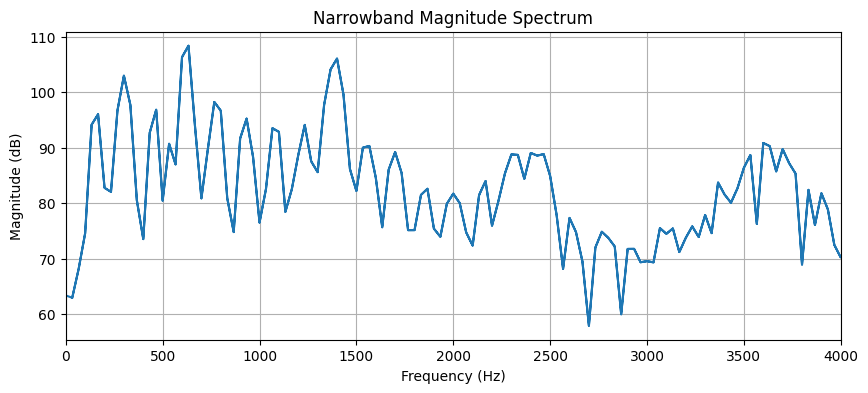
\includegraphics[scale = 0.5]{mag.png}
\end{center}
\end{figure}


\section{Question 3}
With the same 30 ms segment of part 2, compute the autocorrelation coefficients required for the LPC calculation up to p=10. Use the Levinson-Durbin recursion to compute the LP coefficients from the autocorrelation coefficients for each order p = 2,4,6,8,10. Plot error signal energy (i.e. square of gain) vs p.

\subsection{Solution 3}
Using the recursion algorithm that was seen in the class, computed the LP coefficients for each order p.

\subsection{Code}
The code files are included in the .ipynb file included in the submission.

\subsection{Plots}

\begin{figure}[H]
\begin{center}
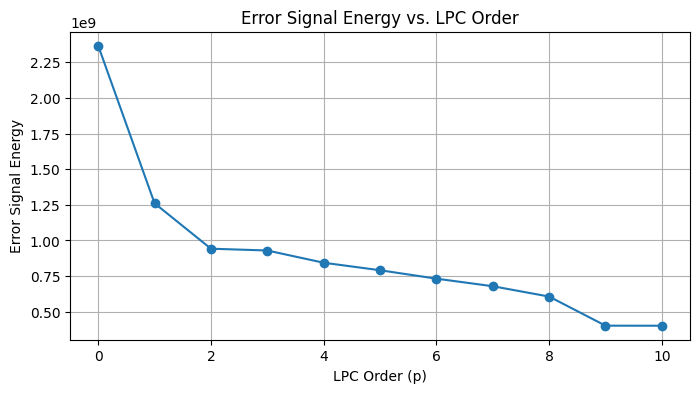
\includegraphics[scale = 0.5]{err.png}
\end{center}
\end{figure}

\subsection{Observations}
We observe that the error continuously decreases as we increase the value of p which was expected.

\section{Question 4}
Show the pole-zero plots of the estimated all-pole filter for p=6,10; comment.


\subsection{Code}
The code files are included in the .ipynb file included in the submission.

\subsection{Plots}

\begin{figure}[H]
\begin{center}
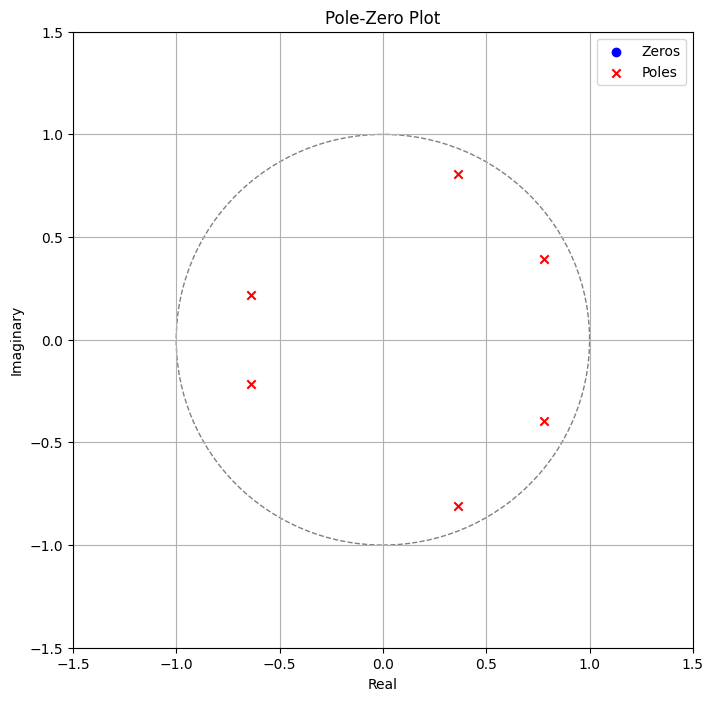
\includegraphics[scale = 0.8]{p6.png}
\end{center}
\end{figure}

\begin{figure}[H]
\begin{center}
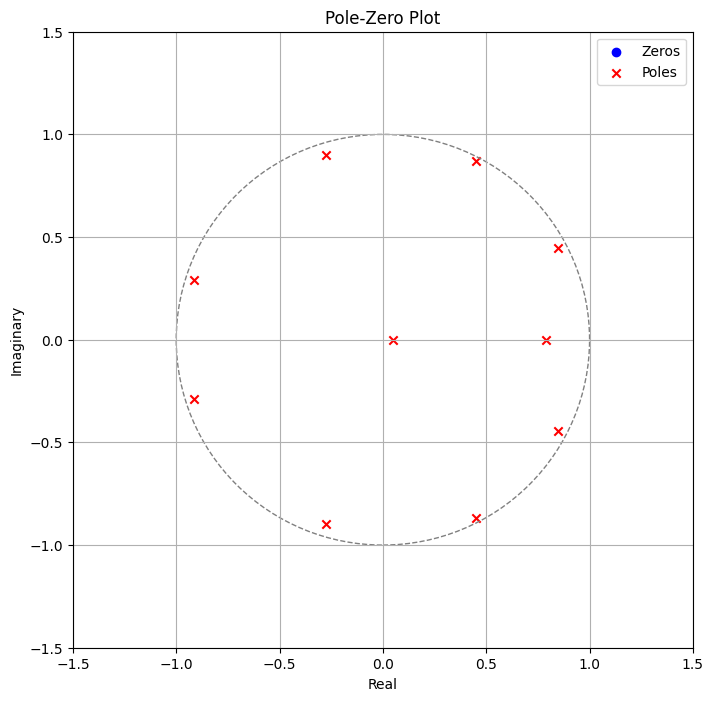
\includegraphics[scale = 0.8]{p10.png}
\end{center}
\end{figure}

\subsection{Observations}
\begin{itemize}
\item For p = 6, we get 6 poles in the pole zero plot. In order to recalculate the formant frequencies and bandwidths of these formants, it has identified three formants whose phase and magnitude can be used. Since the z-plane poles' radius is farther from the unit circle in this situation, their bandwidth spread would be wider.

\item For p = 10, we get 10 poles in the pole zero plot. Therefore we observe that the poles are nearly coinciding on the unit circle meaning that we can more accurately calculate the actual bandwidths.

\end{itemize}



\section{Question 5}
Compute the gain and plot the LPC spectrum magnitude (i.e. the dB magnitude frequency response of the estimated all-pole filter) for each order "p". Comment on the characteristics of the spectral envelope estimates. Comment on their shapes with reference to the short-time magnitude spectrum computed in part 2.



\subsection{Code}
The code files are included in the .ipynb file included in the submission.

\subsection{Plots}

\begin{figure}[H]
\begin{center}
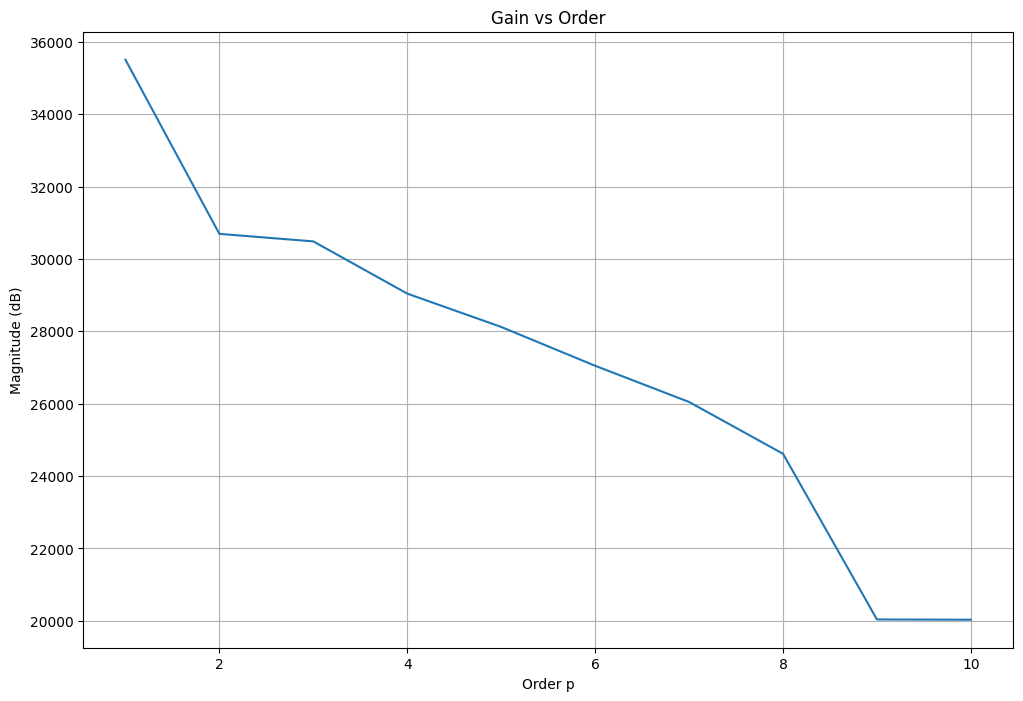
\includegraphics[scale = 0.5]{gain1.png}
\end{center}
\end{figure}

\begin{figure}[H]
\begin{center}
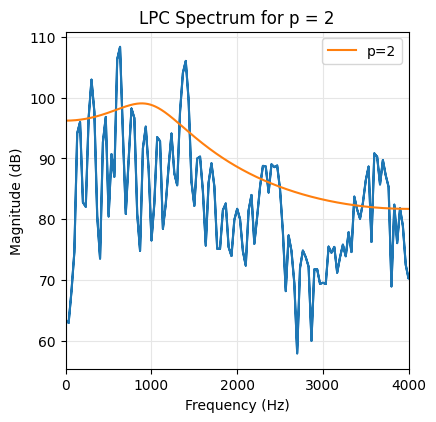
\includegraphics[scale = 0.8]{2p.png}
\end{center}
\end{figure}

\begin{figure}[H]
\begin{center}
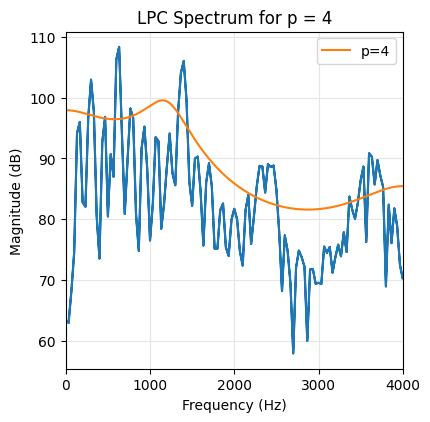
\includegraphics[scale = 0.8]{4p.png}
\end{center}
\end{figure}

\begin{figure}[H]
\begin{center}
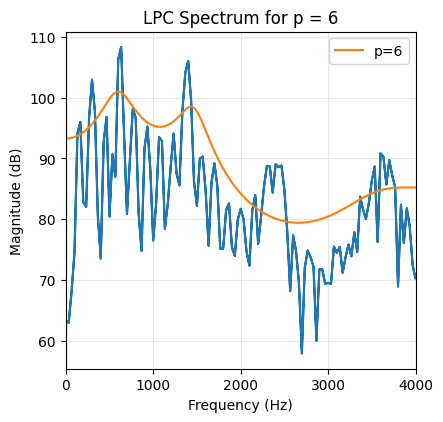
\includegraphics[scale = 0.8]{6p.png}
\end{center}
\end{figure}

\begin{figure}[H]
\begin{center}
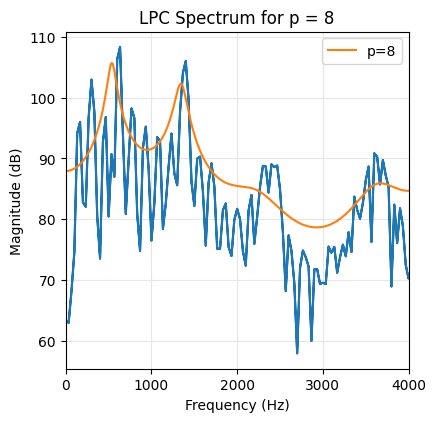
\includegraphics[scale = 0.8]{8p.png}
\end{center}
\end{figure}

\begin{figure}[H]
\begin{center}
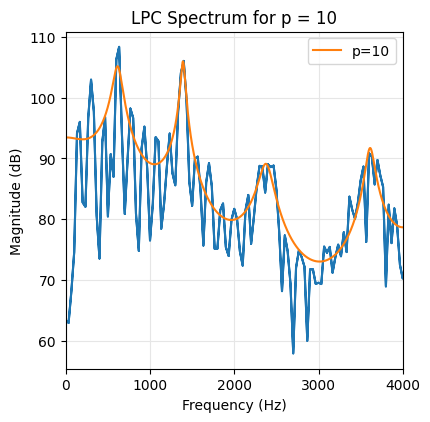
\includegraphics[scale = 0.8]{10p.png}
\end{center}
\end{figure}



\subsection{Observations}
\begin{itemize}
\item We can easily observe that as the order of LPC coefficients increase we are more accurately reaching the actual magnitude spectrum.
\item Also we observe that the gain keeps on decreasing with increasing order because it is directly proportional to the square root of energy so since energy decreases continuously the gain also decreases.
\item Number of formants also increase as we increase the order p.
\end{itemize}

\section{Question 6}
Based on the 10th-order LP coefficients, carry out the inverse filtering of the /a/ vowel segment to obtain the residual error signal. Can you measure the pitch period of the voiced sound from the residual waveform? Use the acf to detect the pitch. Compare the acf plots of the original speech and residual signals.


\subsection{Code}
The code files are included in the .ipynb file included in the submission.

\subsection{Plots}

\begin{figure}[H]
\begin{center}
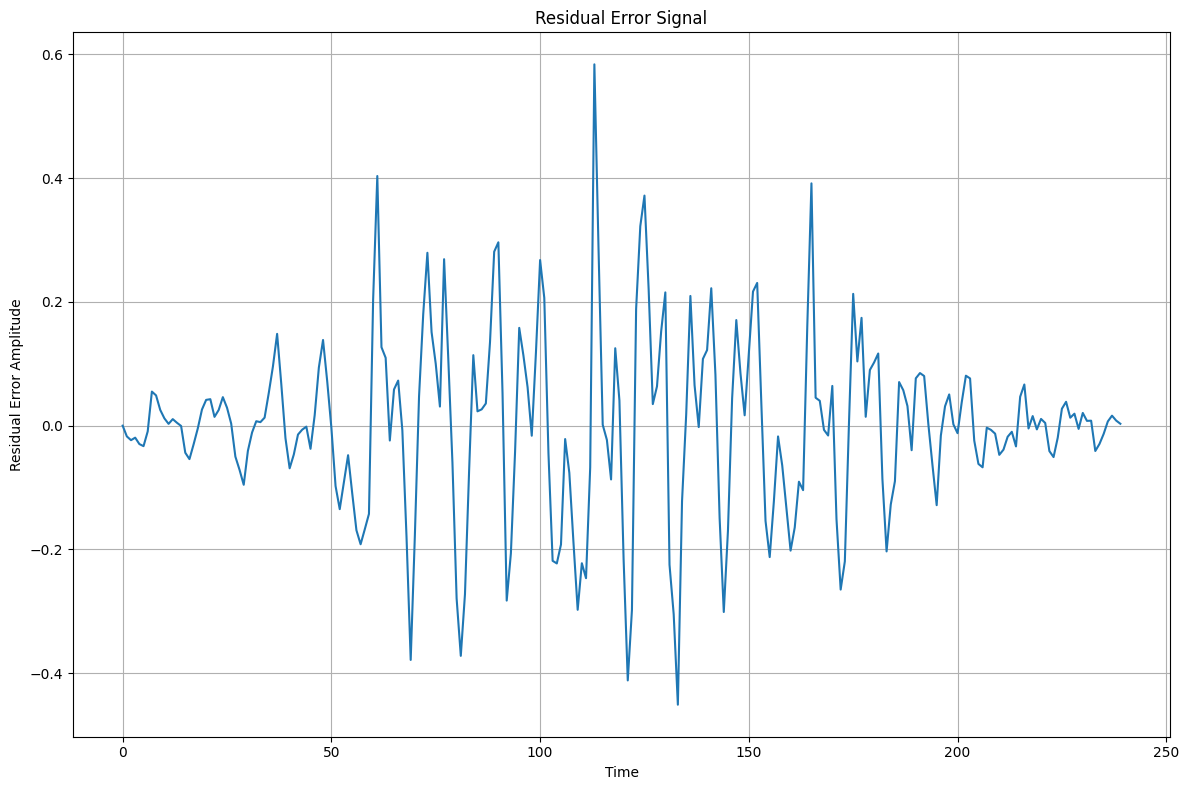
\includegraphics[scale = 0.5]{res.png}
\end{center}
\end{figure}

\begin{figure}[H]
\begin{center}
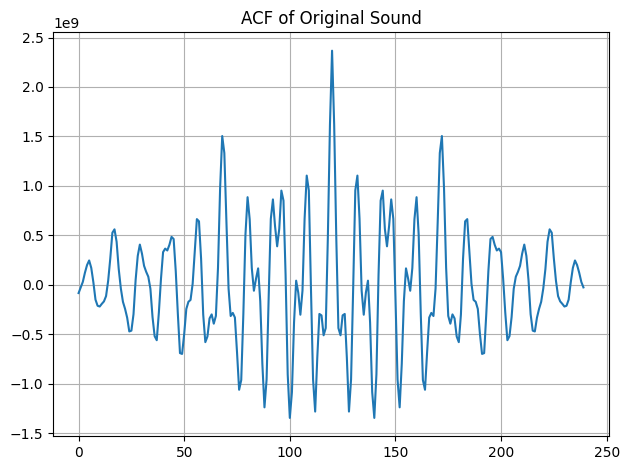
\includegraphics[scale = 0.8]{acf_act.png}
\end{center}
\end{figure}

\begin{figure}[H]
\begin{center}
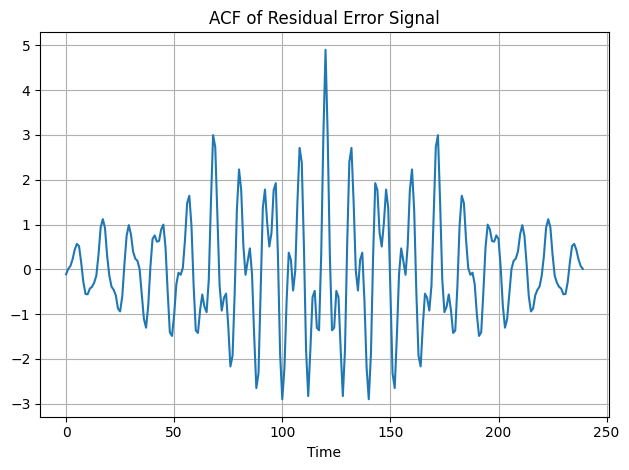
\includegraphics[scale = 0.8]{acf_err.png}
\end{center}
\end{figure}

\subsection{Observations}
\begin{itemize}
\item Yes, we can measure the pitch period of the voiced sound from the residual signal as shown in the code by using the distance between 2 consecutive maximas.
\item Also the shape of Original and Residual Signal is almost same except the magnitude which means that the actuala nd predicted signal is almost same.
\item The pitch calculated by the code in this assignment is 153 Hz approx.
\end{itemize}

\section{Question 7}
LP re-synthesis: We analysed a natural speech sound /uh/ above. Using a suitable set of parameter estimates as obtained there, we wish to reconstruct the sound.\\

That is, use the best estimated LP filter with an ideal impulse train of the estimated pitch period as source excitation. Carry out de-emphasis on the output waveform. Set the duration of the synthesized sound to be 300 ms at 8 kHz sampling frequency and view the waveform as well as listen to your created sound.\\

Comment on the similarity with the original sound. Try out voice modification using this analysis-synthesis method (e.g. change the voice pitch).


\subsection{Code}
The code files are included in the .ipynb file included in the submission.

\subsection{Plots}

\begin{figure}[H]
\begin{center}
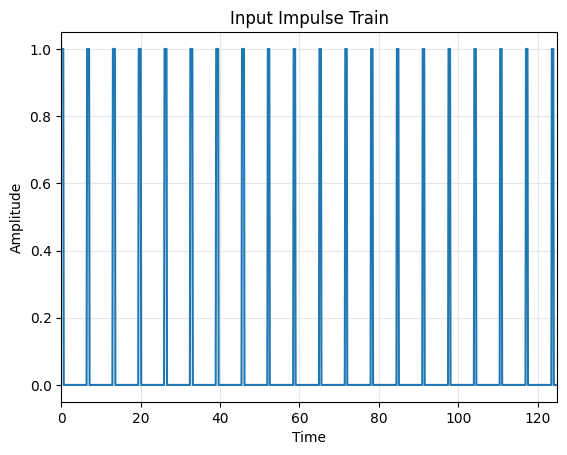
\includegraphics[scale = 0.8]{imp.png}
\end{center}
\end{figure}

\begin{figure}[H]
\begin{center}
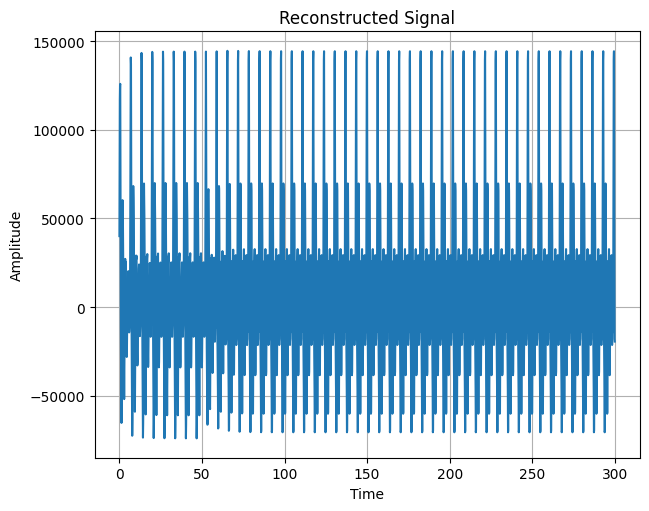
\includegraphics[scale = 0.5]{rec.png}
\end{center}
\end{figure}

\subsection{Observations}
\begin{itemize}
\item After calculating the impulse train we apply that on the signal and then apply de-emphasis because we were working on the emphasis signal from start.
\item The reformed sound is almost similar to the actual sound.
\end{itemize}


\section{Question 8 (BONUS)}

Perform LP analysis on the provided /s/ sound (sampled at 16 kHz).


\subsection{Code}

The code files are included in the .ipynb file included in the submission.

\subsection{Plots}

\begin{figure}[H]
\begin{center}
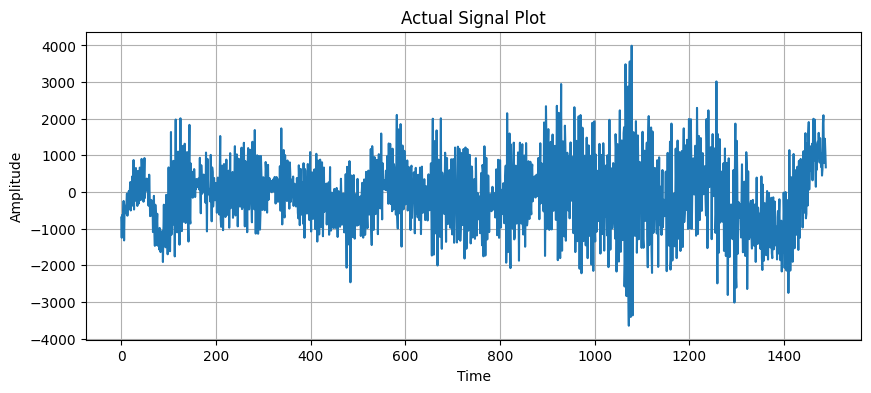
\includegraphics[scale = 0.5]{act2.png}
\end{center}
\end{figure}

\begin{figure}[H]
\begin{center}
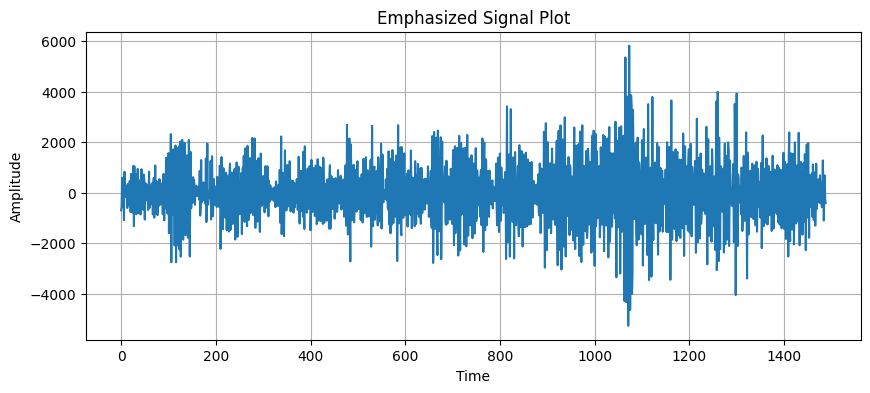
\includegraphics[scale = 0.5]{emph2.png}
\end{center}
\end{figure}

\begin{figure}[H]
\begin{center}
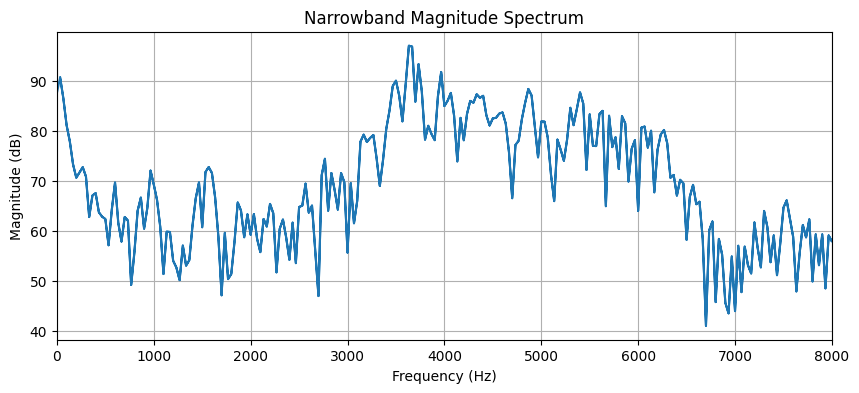
\includegraphics[scale = 0.5]{mag2.png}
\end{center}
\end{figure}

\begin{figure}[H]
\begin{center}
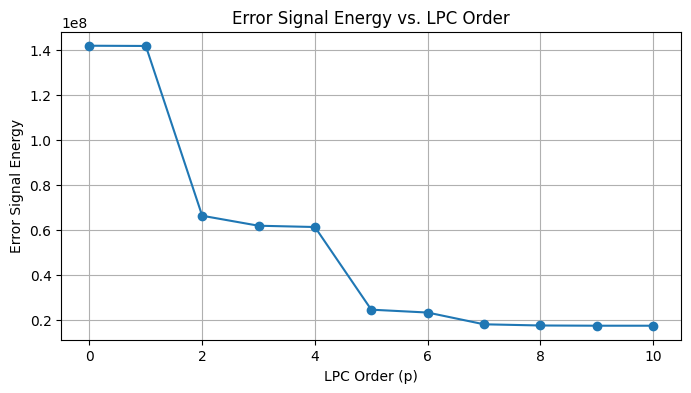
\includegraphics[scale = 0.5]{err2.png}
\end{center}
\end{figure}

\begin{figure}[H]
\begin{center}
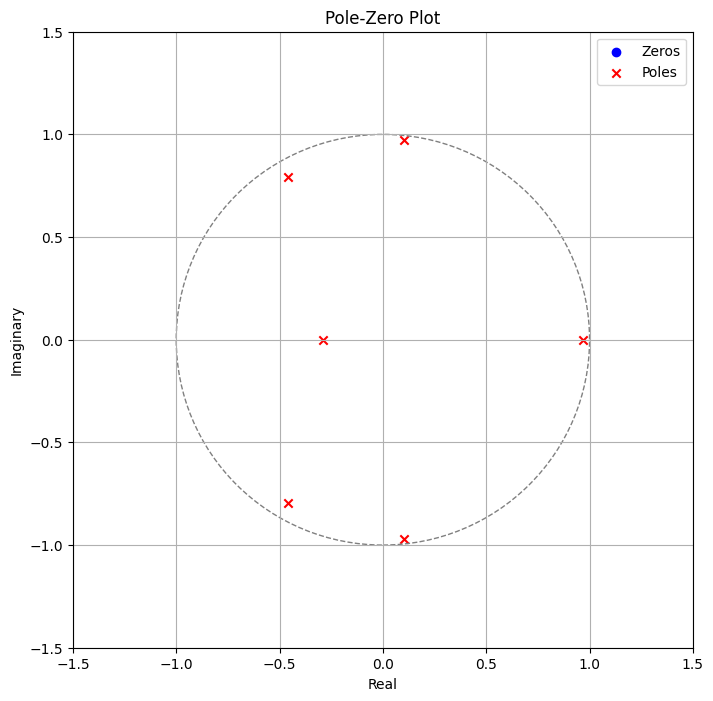
\includegraphics[scale = 0.8]{p6_2.png}
\end{center}
\end{figure}

\begin{figure}[H]
\begin{center}
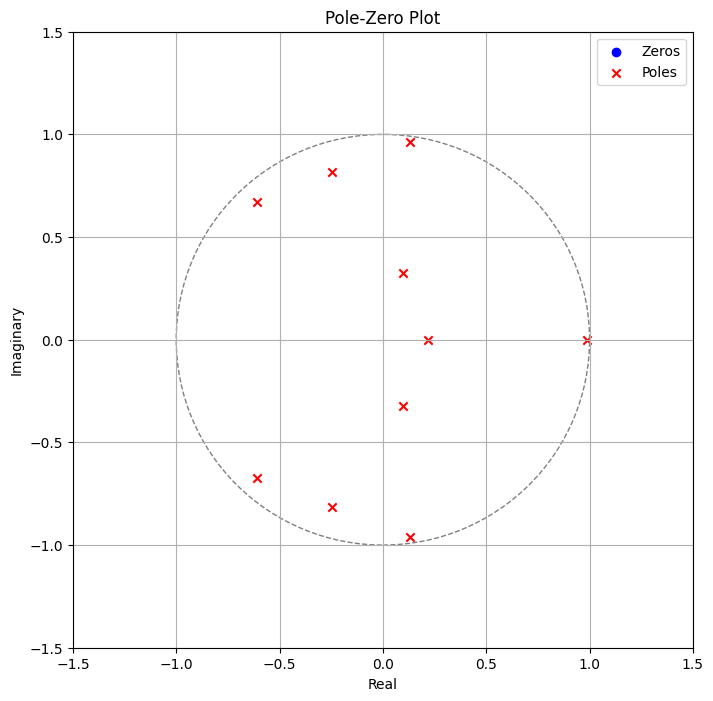
\includegraphics[scale = 0.8]{p10_2.png}
\end{center}
\end{figure}

\begin{figure}[H]
\begin{center}
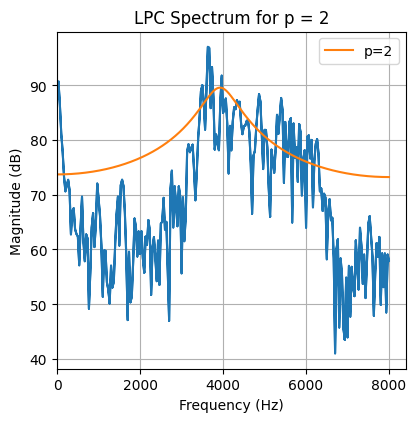
\includegraphics[scale = 0.8]{2p2.png}
\end{center}
\end{figure}

\begin{figure}[H]
\begin{center}
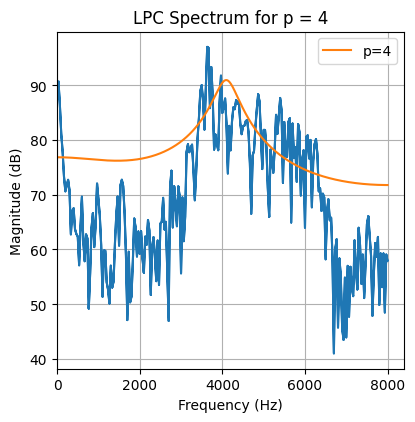
\includegraphics[scale = 0.8]{4p2.png}
\end{center}
\end{figure}

\begin{figure}[H]
\begin{center}
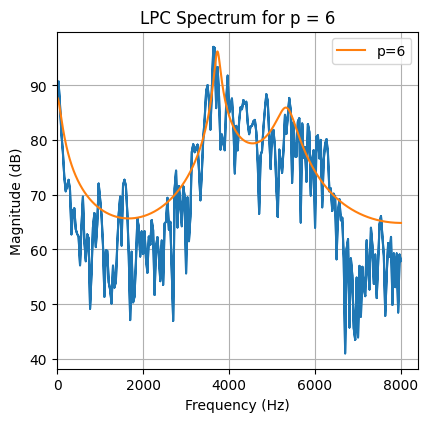
\includegraphics[scale = 0.8]{6p2.png}
\end{center}
\end{figure}

\begin{figure}[H]
\begin{center}
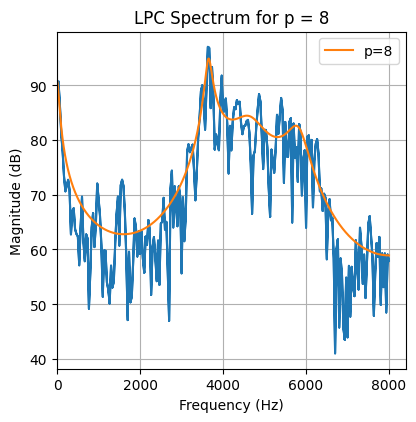
\includegraphics[scale = 0.8]{8p2.png}
\end{center}
\end{figure}

\begin{figure}[H]
\begin{center}
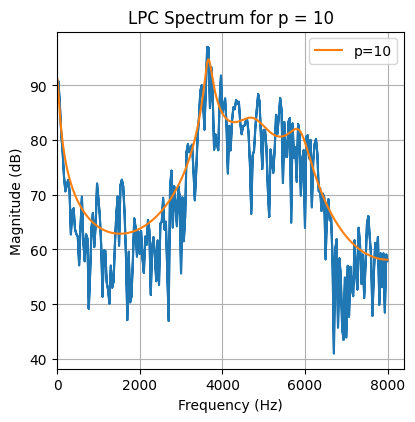
\includegraphics[scale = 0.8]{10p2.png}
\end{center}
\end{figure}

\begin{figure}[H]
\begin{center}
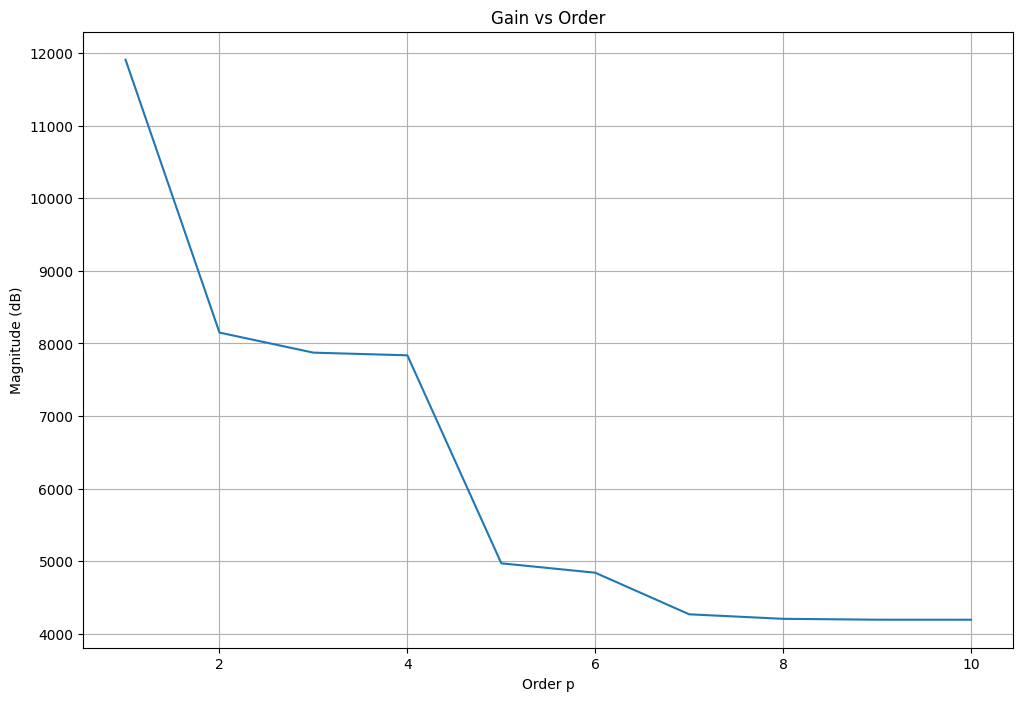
\includegraphics[scale = 0.5]{gain2.png}
\end{center}
\end{figure}

\begin{figure}[H]
\begin{center}
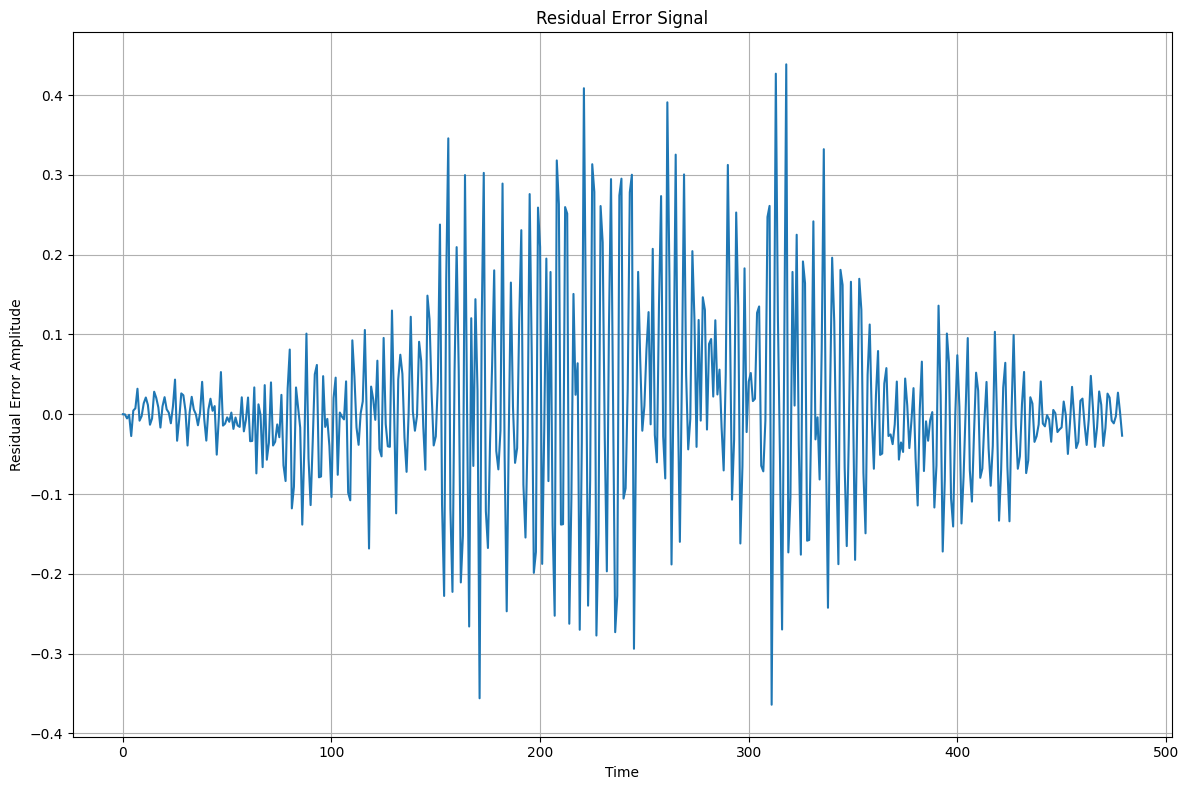
\includegraphics[scale = 0.5]{res2.png}
\end{center}
\end{figure}

\begin{figure}[H]
\begin{center}
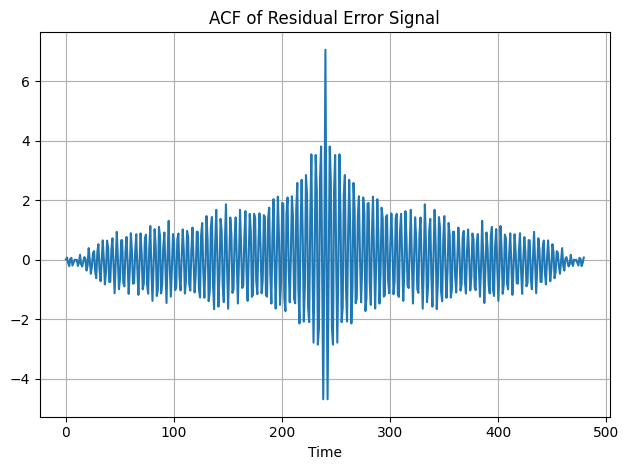
\includegraphics[scale = 0.8]{acf_err2.png}
\end{center}
\end{figure}

\begin{figure}[H]
\begin{center}
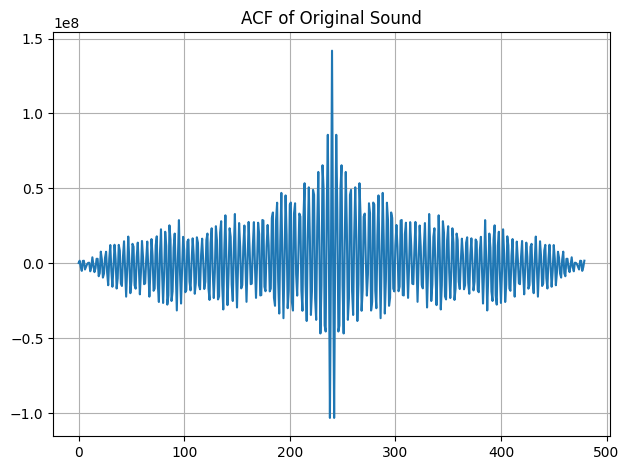
\includegraphics[scale = 0.8]{acf_act2.png}
\end{center}
\end{figure}

\begin{figure}[H]
\begin{center}
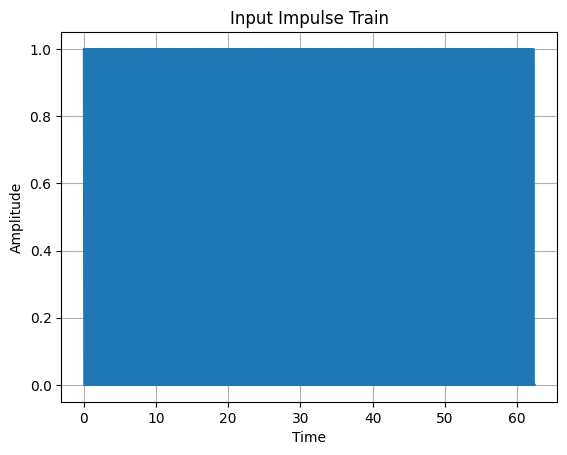
\includegraphics[scale = 0.8]{imp2.png}
\end{center}
\end{figure}

\begin{figure}[H]
\begin{center}
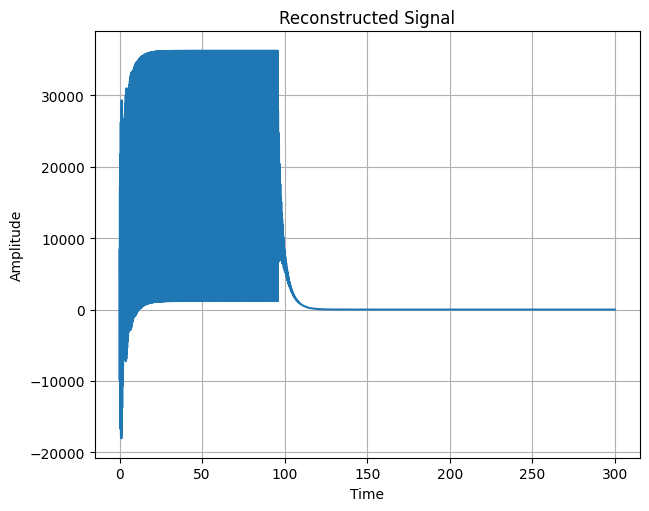
\includegraphics[scale = 0.8]{rec2.png}
\end{center}
\end{figure}

\subsection{Observations}
Now we apply all the things we have done in this assignment to a new audio signal which is given here and the results can be seen in the notebook. We can't calculate the pitch accurately from the second signal i.e. the s sound because it is an unvoiced signal



\end{document}